\chapter{Design Discussion}
\label{ch:design}

\vspace{-1cm}
\begin{center}
Eduard Hirsch and Paolo Dini
\end{center}

\section{ASIM and blockchain}
\label{sec:asim}

Creating a scalable distributed application is a big challenge. Even more so when monolithic legacy systems need to be addressed as in the case of the Sardex payment system, partly realised in Sardinia. For INTERLACE this meant dealing with a system which is currently stable and working reliably. One of the drawbacks of this system, however, is that it does not scale well, which has become increasingly evident in recent times. This problem has become increasingly evident as more circuits from other parts of Italy have been added to the database.

This report describes a prototypical solution of how distribution and scalability are handled using technologies that allow a mutual credit system to grow and evolve. More specifically, for INTERLACE a well-tested architectural, specification, and modelling process was introduced, the Abstract States (Interaction) Machines paradigm \cite{BoergerStaerk2003}, which uses a distributed computational model that allows for iterative refinement of different concurrent and communicating system components in a very specific and detailed way.

As described in \cite{INTERLACE_D21}, an ASIM definition was developed which acts as a ground model for the INTERLACE prototype. This paper-based definition was then transformed into executable code realised with the ICEF,\footnote{Interaction Computing Execution Framework} which is based on ASM language primitives \cite{BoergerStaerk2003}. The implementation, which is the main focus of this report, is the last step before testing, which needs to be done on various levels (component and field testing).

In the following subsections the various topics and challenges encountered during the planning and the definition of the new blockchain-based system are addressed.

\subsection{From Servers to Agents and Peers}

INTERLACE encourages not just a change in technology but also an architectural culture change. Currently many systems in industry are based on monolithic approaches which are stable and based on commonly known and widely adopted implementation strategies. Often not even based on multiple tiers, such classic strategies suit the needs of small and middle-sized projects but come at high cost for very large application services and their providers. When increasing in size they become increasingly difficult to manage given
\begin{quote}
\begin{packed_item1}
	\item their large code base,
	\item non-autonomous teams,
	\item lack in agility,
	\item difficult deployments and
	\item high commitment to specific technologies or even worse vendor lock-ins.
\end{packed_item1}
\end{quote}

Modern large-scale architectures, therefore, aim to find different possibilities in the field of SOA\footnote{Service-Oriented Architecture \cite{erl2014next}}, and when advancing further also in Micro Services Architectures (MSAs). In particular, MSAs \cite{newman2015building} claim to solve these problems by providing simple and easy-to-build applications at the expense of higher network load and more difficult system integration.

However, as mentioned above INTERLACE favours a different solution which has similar ideas but is in some of its most fundamental aspects very different; namely, the blockchain. Although the blockchain, like MSA, has a highly distributed nature, MSA is mainly an architectural stile whereas most blockchains are based on a data-centric approach and are quite specific in terms of scenarios of use. In addition, as discussed more fully in D2.2 \cite{INTERLACE_D22}, permissionless blockchain are also decentralised, which generally refers to a distribution of control in addition to a distribution of the computation. Although in this report we discussed the Hyperledger blockchain, which is permissioned, Hyperledger also has an interface to Ethereum, which is permissionless and which could be a useful addition to the Sardex/INTERLACE platform for example to record currency exchange transactions between circuits in different parts of the world that are pegged 1-1 to different fiat currencies. Finally, in the future an interface to Holochain, which is agent-centric and not data-centric, could also become relevant and useful \cite{INTERLACE_D22,INTERLACE_D23}.

As discussed more fully in \cite{INTERLACE_D22}, desirable properties of blockchain technologies for INTERLACE are:
\begin{quote}
\begin{itemize}
	\item Distribution
	\item Peer to Peer communication
	\item Immutable $\Rightarrow$ auditable 
	\item Data storage
	\item Virtual Machine-like executions of code (chaincode or Smart Contracts)
\end{itemize}
\end{quote}

Further, the use of Smart Contracts or chaincode (Hyperledger Fabric nomenclature) comes with various other attributes which are important to manage a mutual credit system. Code executions which run ``on chain'' are executed on every peer in the network. In order to be executed correctly a blockchain framework defines the roles of various system components, the state of the chain, and the code which is attached to a transaction and takes care of the business logic. The whole framework results in a workflow whose main steps are recorded and written to the blockchain.

Because the technology currently used by Sardex is mainly monolithic, it would be extremely difficult and risky to set up a complete distributed blockchain environment and swap systems from one day to the next. Rather, a roadmap to a completely distributed scenario is being planned, keeping in mind that the code base cannot be changed all at once. In fact, some of the functions of the original system are gradually being reimplemented as external microservices such as, for example, Search. Risk refers to the fact that the non-functional requirements of most blockchain frameworks are still evolving as the technology itself undergoes a continuous process of innovation. In addition, risk also refers to the continuous evolution and innovation that the business model of Sardex itself undergoes. Since blockchains are quite different application platforms which carry certain implications for how users should interact with the software product, any changes in the underlying framework or in the business/application layer need to be introduced gradually and carefully.

Consequently, the INTERLACE focus has been on understanding the complete core requirements, facilitating the AS(I)M approach, creating a generic model, and as much as possible remaining independent of the underlying technology used, in order to make the transition towards a fully distributed, scalable, and reliable system clearer and with minimum risk. For INTERLACE this meant, further, that the agent-based ASIM methodology was used to specify a client-server model to create a Hyperledger Composer-based implementation.

The Hyperledger Composer business network is a blockchain architecture that also incorporates a Micro Services Architecture. Although this is not yet a fully distributed or decentralised scenario, it is scalable because new nodes can be added when extending to other circuits and the transaction processing load can be balanced between them. The permissioned Hyperledger architecture, therefore, allows better control of the blockchain functionalities and the enforcement of rules (business or otherwise), which would otherwise be very difficult or impossible to impose in a permissionless, public chain.

\subsection{Testing}

This subsection gives a quick overview of how testing may be processed for the prototype as well as for the final product. Detailed testing and a description of the testing activities will be reported in D4.1 and D4.2, which will be completed after the end of the project.

There are several levels of testing that need to take place. Since the requirements were defined in the ASIM language and were translated into an ICEF/coreASIM implementation, the test should take this intermediate implementation into account to verify the correctedness system. This, in fact, is integral to the iterative refinement process of the ASM methodology \cite{BoergerStaerk2003}. Traditional approaches like the v-model \cite{forsberg1991relationship} usually test on four levels:
\begin{quote}
\begin{packed_item1}
	\item Acceptance Testing
	\item System Testing
	\item Integration Testing
	\item Unit Testing
\end{packed_item1}
\end{quote}

ASIM ground model testing cannot be put into one of these categories directly. Further, under the umbrella of modern software development methods like (large-scale) scrum, (scaled) agile different testing practices have been adopted besides the traditional approaches.

For D4.1/2 it is planned to test based on the results of the execution of the ASIM Models. Thus, each of the requirements has a specific output, which is then compared to the log of an execution produced by the new system. This is of course a pretty high-level way of testing. Compared to traditional testing it may be seen to lie between Integration and System Testing, but not properly in the realm of acceptance testing since the requirements defined by ASIMs are mathematically-based algorithms which are difficult to read and to verify by non-technical people.

Cucumber\footnote{\url{https://cucumber.io}} may be used as a potential replacement tool for the ASIM comparison testing. Cucumber is a scenario-based testing tool which combines functional requirements into high-level system tests which are described as text as well as with a domain-specific language that enables the exectution of the test. A testing scenario may look like the one shown in Listing \ref{lst:cucumber}.

\begin{center}
\begin{minipage}{0.8\textwidth}
\small
\begin{lstlisting}[language=cucumber,firstnumber=1,caption={\bf\small Cucumber test example},captionpos=b,label=lst:cucumber]
Feature: Perform Credit operations
  Move money from an account of member A to an account of member B
  
  Scenario: account B receives 100 Sardex from account A
    Given: Account A has a positive balance
      And: Account B is able to receive money
      And: Account A has a balance of 100
      And: Account B has a balance of 0
     When: Credit Transaction has performed successfully
     Then: account A has a balance of 0
      And: account B has a balance of 100
\end{lstlisting}
\end{minipage}
\end{center}

The various steps $Given$ [initial context], $When$ [event occurs], $Then$ [ensure some outcomes] are based on a special language called Gherkin\footnote{\url{https://docs.cucumber.io/gherkin}} whose elements can be connected to test implementations serving that scenario. Details can be found in the publicly available Cucumber documentation.
  
\section{Solution Technologies}
\label{sec:solution}

This last introductory part finally presents the planned solution stack which will be utilised for the prototypical implementation and is illustrated in Figure \ref{fig:solution-stack}. Details on how these components work together are explained in depth in Section \ref{ch:prototype}.

\begin{figure}[htbp]
  \centering
  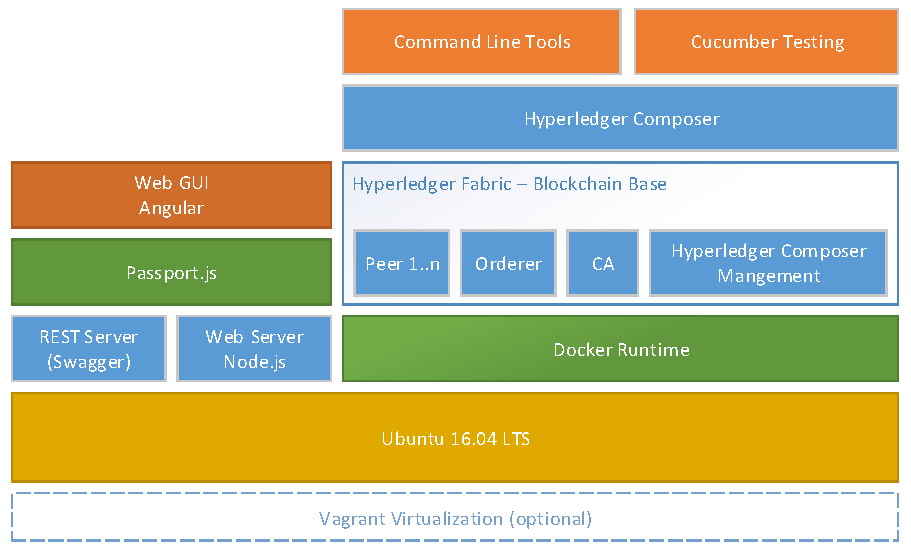
\includegraphics[width=1.0\textwidth, clip, trim=1mm 1mm 1mm 1mm]{Figures/solution-stack}
  \caption{\bf\small Technologies involved for the final solution stack}
  \label{fig:solution-stack}
\end{figure}

Although detailed explanation will be given in Section \ref{ch:prototype}, a simple structure introduction is given here.

The whole system currently runs on Ubuntu Version 16.04 LTS as Hyperledger Fabric together with Composer work properly only on the MacOs or Linux operating systems. Thus, optionally, a possibility exists which includes virtualizsation. On GitHub\footnote{\url{https://github.com/hirsche/hyperledger}} a Vagrant-assisted Hyper-V or VirtualBox Machine may be started providing an Ubuntu 16.04 ecosystem, which is also explained in the next section.

On top of Ubuntu a Docker runtime hosts a Hyperledger Fabric docker-compose cluster which runs one to $n$ peers, an Orderer, and a Certification Authority (CA), as well as managing a container which handles the Hyperledger Composer-specific part.

This base Fabric environment is managed by the Composer wrapper framework, which forms the key access port for the other components and provides help during implementation and the setting up of a business network.

Next, the Composer API provides stubs for the REST Server and the Web Server implementations, which really simplifies the programming necessary. These servers can be used to first load the application and connect it to the business network, and then execute various transactions/transfers. The Web Application is implemented using AngularJS and may be secured using Passport.js, which is an authentication middleware.

Finally, on top of the whole stack, Cucumber tests can be used to verify simple scenarios.


